%**************************************************************
% Lab 09: ROM
%**************************************************************
\chapter{ROM}\label{Lab09}

\section{Purpose}

\begin{wrapfigure}{O}{0.2\textwidth}
	\caption*{} % No text, wraps badly in very narrow space (does print fig number)
	% to not print a fig number use \caption*{}
	\label{fig:09-01} 
	\centering
	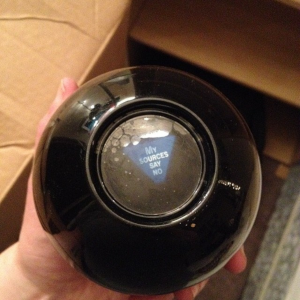
\includegraphics[width=0.2\textwidth]{gfx/09-01} 
\end{wrapfigure}
This lab introduces students to \acf{ROM} and builds a fun application: The \textit{Magic 8-Ball}. This was a toy that was developed in the 1950s and was popular throughout the 1960s. It was a small plastic sphere with the markings of an 8-ball. If the user ``asked it a question'' and then turned the toy upside down the answer would magically appear in a small window on the bottom of the ball.

\section{Procedure}

Start a new \LE project and create a subcircuit named \lstinline[columns=fixed]|Magic_8_Ball|. Open that circuit and place a ROM (\textit{Memory} library) device near the center of the drawing canvas. Set the ROM properties for an \textit{Address Bit Width} of 12 and a \textit{Data Bit Width} of 8\footnote{The provided starter circuit already contains the \lstinline[columns=fixed]|Magic_8_Ball| subcircuit along with two devices needed in the early part of the build.}.

\begin{figure}[H]
	\centering
	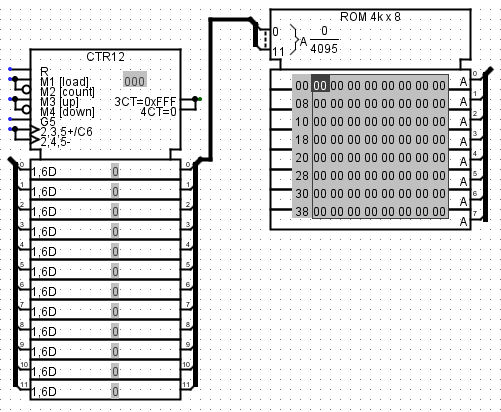
\includegraphics[width=\maxwidth{.95\linewidth}]{gfx/09-02}
	\caption{Placing ROM}
	\label{fig:09-02}
\end{figure}

A ROM stores data that is accessed by setting an address on the inputs at the top left of the device and then reading the contents of that address on the 8-bit bus on the right side of the device. By attaching a counter to the ROM address port several consecutive addresses can be ``stepped through'' to output a message. Attach a Counter (\textit{Memory} library) with 12 Data Bits to the address port of the ROM, as in Figure \ref{fig:09-03}.

\begin{figure}[H]
	\centering
	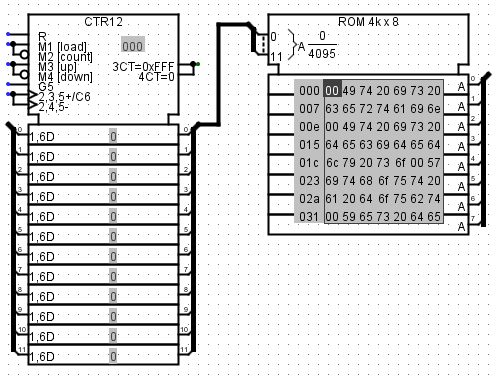
\includegraphics[width=\maxwidth{.95\linewidth}]{gfx/09-03}
	\caption{ROM With Counter}
	\label{fig:09-03}
\end{figure}

According to Wikipedia\footnote{\url{https://en.wikipedia.org/wiki/Magic_8-Ball}}, the Magic 8-Ball featured 20 sayings: 

\begin{verbatim}
 1 001 It is certain
 2 00f It is decidedly so
 3 022 Without a doubt
 4 032 Yes definitely
 5 041 You may rely on it
 6 054 As I see it yes
 7 064 Most likely
 8 070 Outlook good
 9 07d Yes
10 081 Signs point to yes
11 094 Reply hazy try again
12 0a9 Ask again later
13 0b8 Better not tell you now
14 0d1 Cannot predict now
15 0e4 Concentrate and ask again
16 0fe Do not count on it
17 111 My reply is no
18 120 My sources say no
19 132 Outlook not so good
20 146 Very doubtful
\end{verbatim}

The \textit{Magic 8-Ball} simulator built in this lab uses those same 20 saying. In the above chart, each saying is numbered and the start point in ROM (using hexadecimal notation) for each saying is also noted. Thus, saying one starts on ROM byte 001, saying two starts on ROM byte 00f, saying three starts on ROM byte 022, and so forth.

The content of the ROM device must be loaded before it can be used and that content is provided in \emph{\texttt{Lab09\_ROM.txt}} accompanying this lab. To load the ROM device, click it one time and then click the ``(click to edit)'' link in its properties panel. In the ROM editor window that pops up, click the ``open'' button and navigate to the ROM memory file. Click ``close window'' to load the ROM device and make it ready for service\footnote{The ROM device provided with the starter circuit is pre-loaded so it will not be necessary to load it again. However, this information is left here for students who may want to load the ROM for practice.}.

The start point for each saying, as indicated on the above table, is stored in a Constant (\textit{Wiring} library) then a Mux (\textit{Plexers} library) with five select bits is used to transmit a message start location to the counter so it can be read from the ROM device. Figure \ref{fig:09-04} illustrates the circuit at this point\footnote{The multiplexer provided with the starter circuit already has the various constants attached. Students who wish to do so can create their own multiplexer by using the start addresses in the ``Sayings'' listing above.}.

\begin{figure}[H]
	\centering
	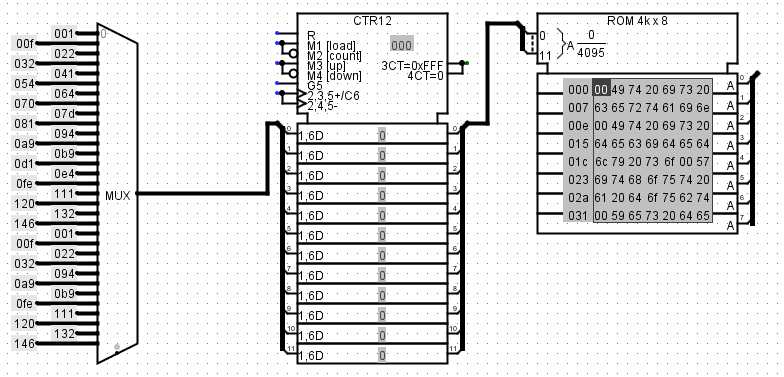
\includegraphics[width=\maxwidth{.95\linewidth}]{gfx/09-04}
	\caption{ROM Filter Mux}
	\label{fig:09-04}
\end{figure}

A five-bit Random Generator (\textit{Memory} library) is used to select a random message. Figure \ref{fig:09-05} illustrates the placement of the random generator.

\begin{figure}[H]
	\centering
	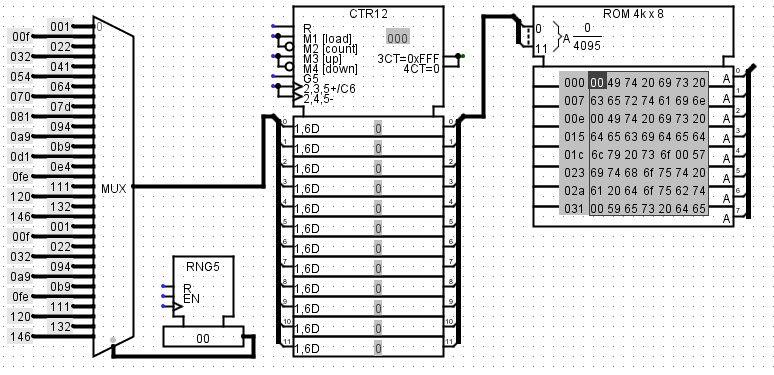
\includegraphics[width=\maxwidth{.95\linewidth}]{gfx/09-05}
	\caption{Random Generator Added}
	\label{fig:09-05}
\end{figure}

To complete the circuit, a few odds-and-ends were added. Figure \ref{fig:09-06} shows the completed circuit, but details from that figure are used below to describe how to complete the circuit.

\begin{figure}[H]
	\centering
	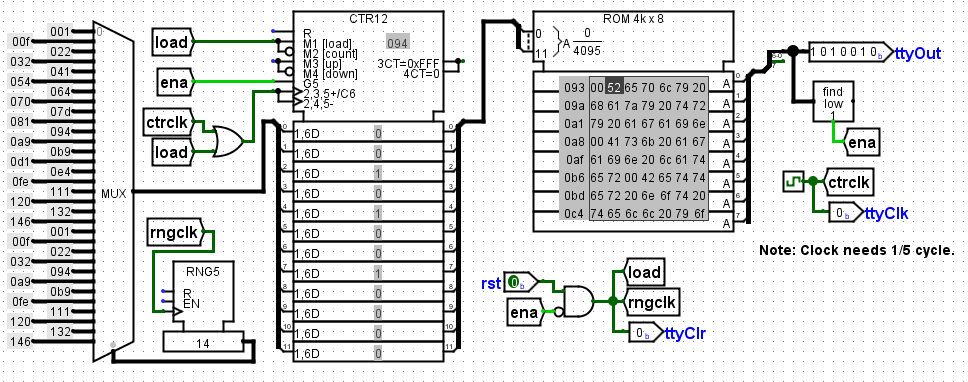
\includegraphics[width=\maxwidth{.95\linewidth}]{gfx/09-06}
	\caption{Completed Magic 8-Ball Circuit}
	\label{fig:09-06}
\end{figure}

To set up the counter, four signals are needed. These are all from tunnels (\textit{Wiring} library) connected to other spots on the circuit. (See Figure \ref{fig:09-07}.)

\begin{itemize}
	\item \textbf{load}. The load signal goes high when the counter should be loaded with a new number from the multiplexer. The number loaded is the location in ROM for the start of a message. Notice that the load signal is used on two pins. The top pin places the counter in load mode while the bottom pin uses the load signal as a clock pulse.
	\item \textbf{ena}. The enable signal turns the counter on/off. When enable is high then the counter functions normally and when it is low the counter is disabled.
	\item \textbf{ctrclk}.The counter clock provides the clock signal for the counter.
\end{itemize}

Connect the random number generator as follows. (See Figure \ref{fig:09-07}.)

\begin{itemize}
	\item The clock input pin is connected to a ``rngclk'' tunnel.
	\item The generator output is wired to the select port of the multiplexer.
\end{itemize}

\begin{figure}[H]
	\centering
	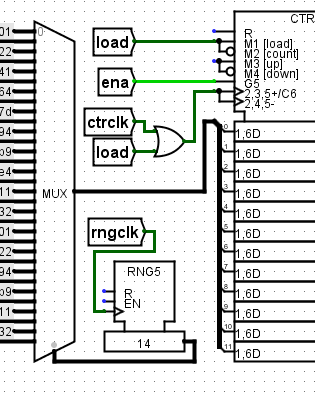
\includegraphics[width=\maxwidth{.95\linewidth}]{gfx/09-07}
	\caption{Counter Inputs}
	\label{fig:09-07}
\end{figure}

The counter control signals are generated and distributed from a small group located under the ROM device. The purpose of this tiny group is to transmit a high signal through the AND gate when the reset pin goes high while enable is low. This generates the signals needed to select a new random message and put the starting address of that message in the counter. (See Figure \ref{fig:09-08}.)
 
\begin{itemize}
	\item \textbf{rst}. The reset pin is an external signal that originates from the \lstinline[columns=fixed]|main| circuit.
	\item \textbf{ena'}. Enable Not originates from the ROM output group.
	\item \textbf{load}. This signal is used to load a message starting address into the counter. When it goes high it activates the ``load'' function and also becomes a single clock pulse for the counter.
	\item \textbf{rngclk}. The random number generator clock signal activates that device so it generates a random number. That number is then used to select a single line from the multiplexer so a message starting address can be loaded.
	\item \textbf{ttyClr}. This sends a high signal to the TTY ``clear'' pin on the \lstinline[columns=fixed]|main| circuit. That signal is used to clear the TTY device.
\end{itemize}

\begin{figure}[H]
	\centering
	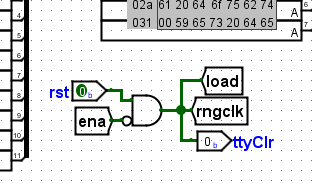
\includegraphics[width=\maxwidth{.95\linewidth}]{gfx/09-08}
	\caption{Counter Control Generation and Distribution}
	\label{fig:09-08}
\end{figure}

There are two functions found at the ROM device output. (See Figure \ref{fig:09-09}.)

\begin{itemize}
	\item The output of the ROM device is connected to the \textit{ttyOut} pin in order to drive the teletype device on the \lstinline[columns=fixed]|main| circuit.\footnote{Note that at the output of the ROM device is a splitter. ASCII letters are only seven bits wide so this splitter passes bits 0-6 to the \textit{ttyOut} port but bit 7 (the most significant bit) is simply discarded. The provided starter circuit includes the splitter.}

	\item The Bit Finder (\textit{Arithmetic} library) attached to the output of the ROM device is used to find the lowest-order \textit{one} in the ROM byte output. If the ROM byte includes at least one \textit{one} then the south port of the finder is high. If the ROM output is all zeros then the Finder output it goes low and that is used as the \textit{ena} signal for the counter and random number generator. When the enable signal is low it also permits a \textit{rst} signal (generated on the \lstinline[columns=fixed]|main| circuit when the user ``asks another question'') to create a new answer.
	
	\item Near the output of the ROM device a clock signal is split to two outputs. One is the \textit{ctrclk} tunnel that is used by the counter and the other is the \textit{ttyClk} pin, which is used on the \lstinline[columns=fixed]|main| circuit to clock the teletype device. \textbf{It is important to note that the clock properties are set for a 1 tick high duration and 5 ticks low duration (a 1/5 clock).}
\end{itemize}

\begin{figure}[H]
	\centering
	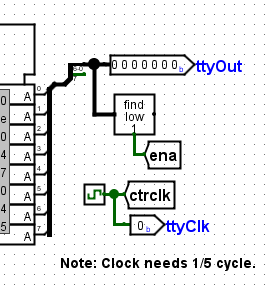
\includegraphics[width=\maxwidth{.95\linewidth}]{gfx/09-09}
	\caption{ROM Output}
	\label{fig:09-09}
\end{figure}

The only remaining step is to create the \lstinline[columns=fixed]|main| circuit. As in all labs in this manual, the \lstinline[columns=fixed]|main| circuit does nothing more than provide a user interface for the \textit{Magic 8-Ball} Circuit. Figure \ref{fig:09-10} illustrates the \lstinline[columns=fixed]|main| circuit.

\begin{figure}[H]
	\centering
	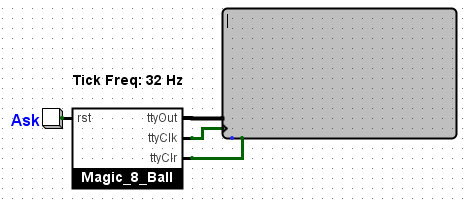
\includegraphics[width=\maxwidth{.95\linewidth}]{gfx/09-10}
	\caption{Magic 8-Ball Main Circuit}
	\label{fig:09-10}
\end{figure}

\subsection{Testing the Circuit}

Before the circuit can be tested the ROM device must be loaded. The ROM was loaded earlier in the lab but in case it does not have any content (it is filled with zeros), then load it with \emph{\texttt{Lab09\_ROM.txt}}, which was provided with the lab. To load the ROM device, click it one time and then click the ``(click to edit)'' link in its properties panel. In the ROM editor window that pops up, click the ``open'' button and find the ROM memory file. Click ``close window'' to load the ROM device and make it ready for service.

The circuit should be tested by enabling the simulator clock at a frequency of 32 Hertz. Every time the \textit{Ask} button is pressed a new random message will be displayed on the teletype screen\footnote{Due to the way this circuit is constructed one out of six button presses will fail and no message will be displayed. The failures are random events so the circuit may fail several times in a row but then not fail for the next 20 or more presses. Students may want to investigate this bug but that is not required.}.

\section{Deliverable}

To receive a grade for this lab, build this circuit. Be sure the standard identifying information is at the top left of the \lstinline{main} circuit, similar to: 

\bigskip
% The minipage environment keeps the three lines together - no page break.
\begin{minipage}{\linewidth}
	\begin{verbatim}
	George Self
	Lab 09: ROM
	September 13, 2019
	\end{verbatim}
\end{minipage}
\bigskip

Save the file with this name: \textit{Lab09\_ROM} and submit that file for grading.

